\section{\text{Въведение}}
\begin{frame}[t]{Комари}
  \begin{figure}[h]
    \centering
    \begin{subfigure}{0.5\textwidth}
      \centering
      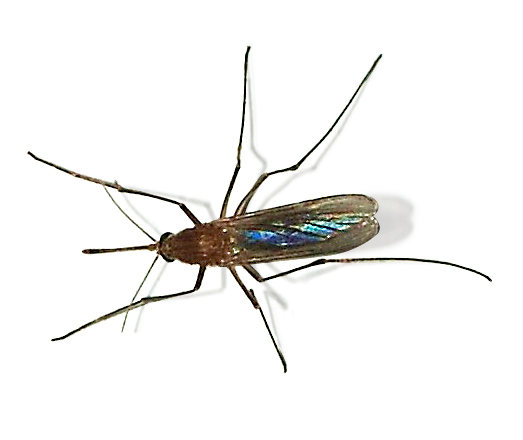
\includegraphics[width=0.5\textwidth]{Culex_pipiens_2007-1.jpg}
      \caption{\textit{Culex pipiens}}
      \label{fig:Culex}
    \end{subfigure}%
    \begin{subfigure}{0.5\textwidth}
      \centering
      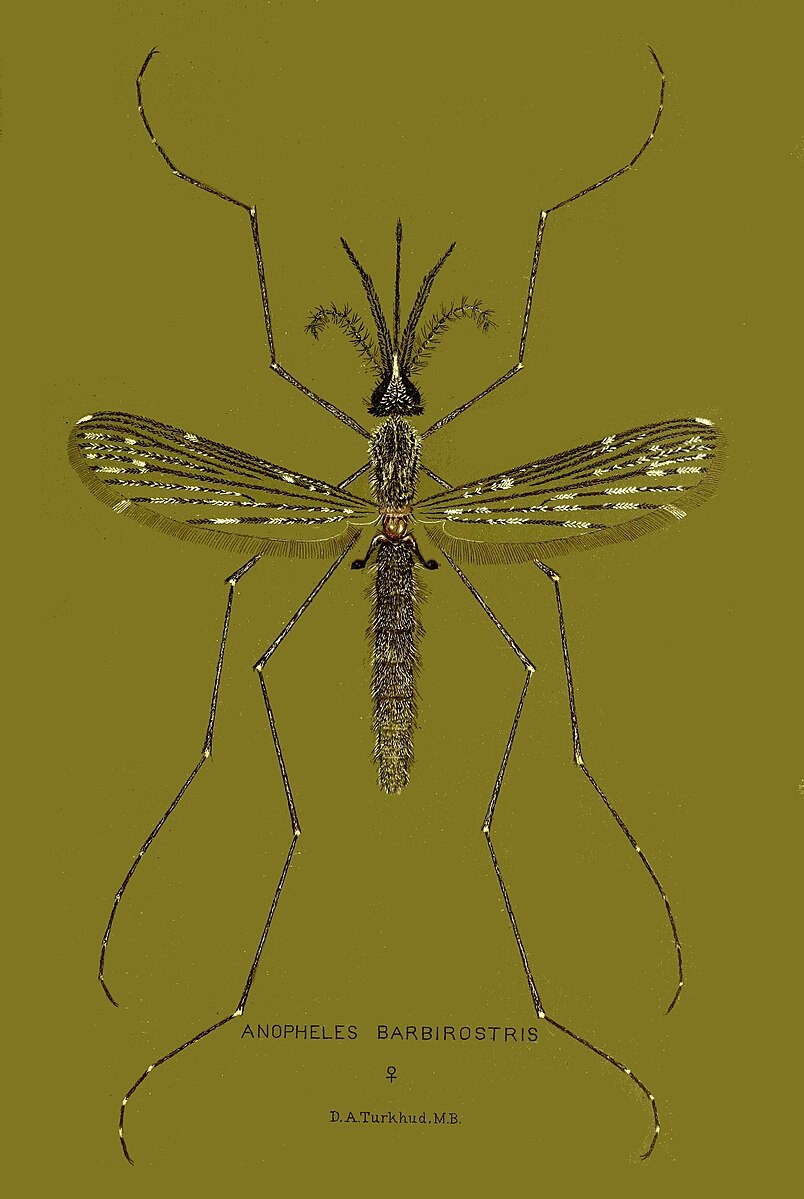
\includegraphics[width=0.5\textwidth]{Anopheles_barbirostris.jpg}
      \caption{\textit{Anopheles barbirostris}}
      \label{fig:Anopheles}
    \end{subfigure}
  \end{figure}
\end{frame}

\begin{frame}[t]{Термини от епидемологията}
  \begin{itemize}
    \item Патоген е причинител на зараза (напр. вирус, бактерия, прион).
    \item Вектор е носител на патоген, който може да зарази други индивиди.
    \item S (Susceptible) - податливи са тези, които не носят патогена и могат да бъдат заразени с него
    \item E (Exposed) - латентни са носители на патогена, които не могат да го предадат
    \item I (Infectious) - заразни са носители на патогена, които могат да го предадат
    \item R (Removed/Recovered/Resistant) - резистентни са тези, които имат (или са получили след заразяване с патогена) имунитет (може да е временен) към патогена и не могат нито да го разпространят, нито да бъдат заразени
  \end{itemize}
\end{frame}

\begin{frame}[t]{Развитие на заразата}
  В зависимост от природата на заразата, могат да се наблюдават различни преходи на индивид от един в друг клас с течение на времето:
  \begin{itemize}
    \item $S \rightarrow E \rightarrow I \rightarrow R \rightarrow S$ (SEIRS)
    \item $S \rightarrow I \rightarrow R$ (SIR) напр. рубеола
    \item $S \rightarrow I \rightarrow R \rightarrow S$ (SIRS)
    \item $S \rightarrow E \rightarrow I$ (SEI) напр. HIV
    \item $S \rightarrow I \rightarrow S$ (SIS) напр. малария, инфлуенца
  \end{itemize}
  Понякога по-сложни заболявания могат да се моделират с по-прости модели (напр. да допуснем, че няма латентна фаза), но тогава няма да получим същата точност при прогноза на развитието на заболяването.
\end{frame}

\begin{frame}[t]{Разпространение на заразата}
  Разглеждат се модели, които разглеждат разпространението на патогена в популация/-и.

  Отчита се факта, че категориите влияят една на друга, например заразните могат да заразят човек от податливите и така той да се причисли към тяхната група.

  Възможно е да имаме повече от една съвкупност от групи SEIRS хора (напр. разделение по възраст, местообитание), за които да имаме различни податливости на патогена.

  Възможно е да имаме повече от една съвкупност от групи SEIRS, отговаряща за различни видове.

  Възможно е да се разглежда популационната динамика при развитие за прогнози далеч във времето.
\end{frame}

\begin{frame}[t]{Малария}
  Патогенът е маларийни плазмодии (едноклетъчни еукариоти, т.е. едноклетъчни с ядро).

  Симптоми са периодичен пароксизъм(продължителни спазми, потене, треска), умора, главоболие, белодробен оток, разрастнал се черен дроб, смърт.

  През XIX са открили връзката с болестта и присъствието на комари, но първоначално се е предполагало, че патогена се пренася по вода.

  Патогенът произхожда от Южна Африка.
  В днешно време маларията се среща в Южна Африка, Югоизточна Азия.
\end{frame}

\begin{frame}[t]{Малариен плазмодий}
  \begin{figure}
    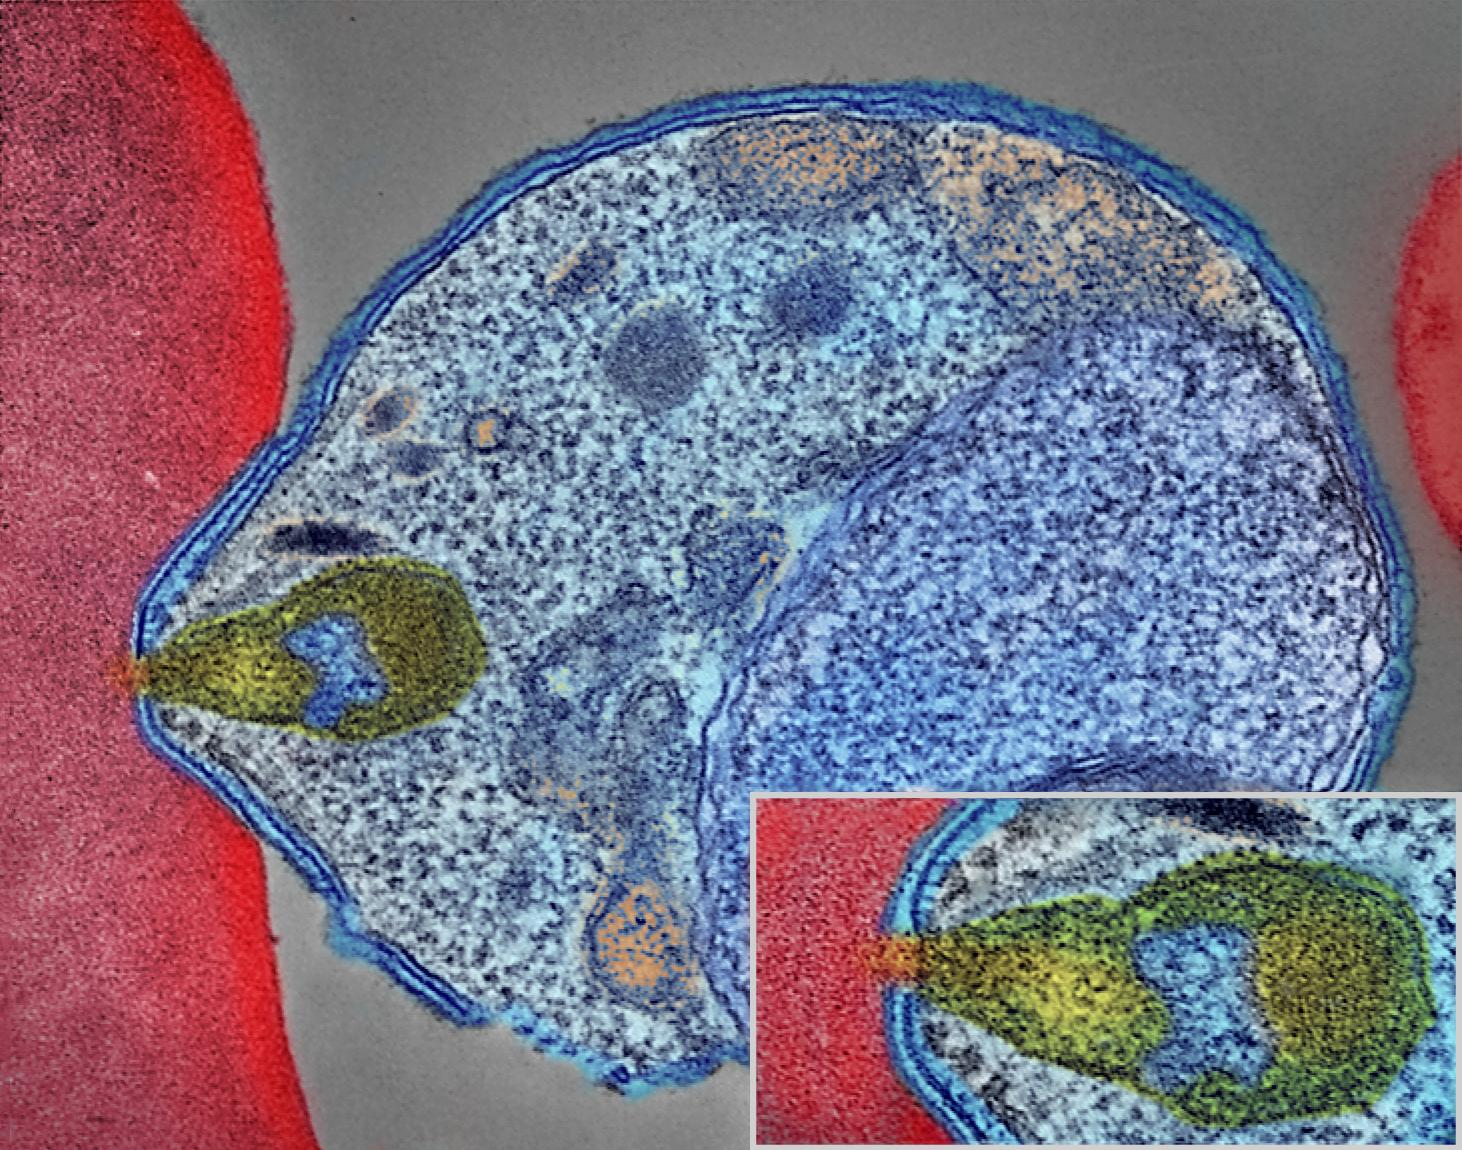
\includegraphics[height=0.6\textheight]{Malaria_Parasite_Connecting_to_Human_Red_Blood_Cell_(34034143483).jpg}
    \centering
    \caption{Оцветена електронно микроскопска снимка на плазмодий нападащ еритроцит}
  \end{figure}
\end{frame}

\begin{frame}[t]{Малариен плазмодий}
  \begin{figure}
    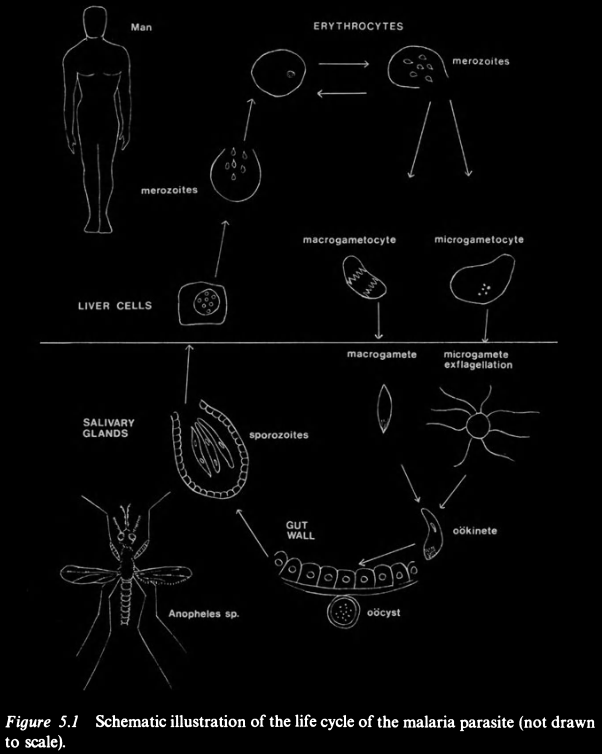
\includegraphics[height=0.75\textheight]{malaria-transmission-negative.png}
    \centering
    \caption{Жизнен цикъл на патогена}
  \end{figure}
\end{frame}

\begin{frame}[t]{Ronald Ross}
  Роден през 1857 в Индия син на английски офицер.

  Получава медицинско образование в Англия, а преди това се образова по многобройни теми, включително математика.

  След поредица експерименти през 90-те години на XIX век, Ronald Ross открива плазмодият в слюнчестите жлези на комари от род Anopheles.

  За приноса си получава става носител на Нобеловата награда за медицина през 1902г.

  Лансира идеята за изтребване на комарите като начин за справяне с маларията.
  За да убеди в това твърдения създава математически модел на маларията и го изследва, като така получава рицарско звание.

  Почива през 1932 г.
\end{frame}

\begin{frame}[t]{Ronald Ross}
  \begin{figure}
    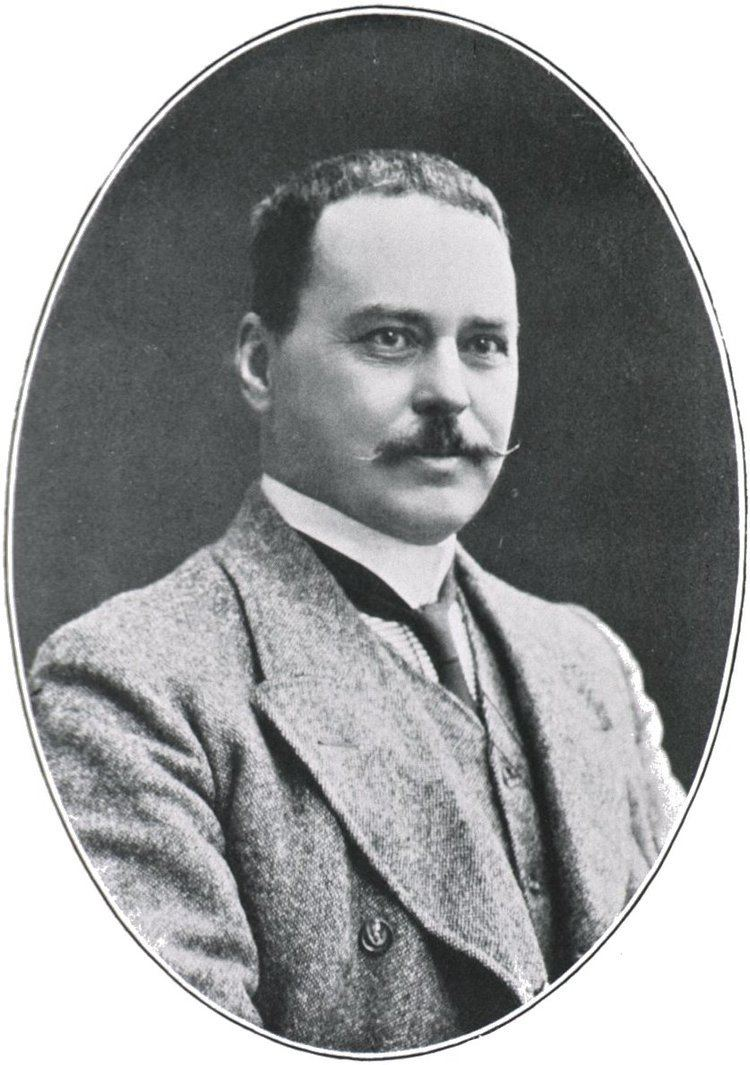
\includegraphics[width=0.7\textwidth, height=0.75\textheight]{ronald-ross-e053ee1d-92ea-4ae9-a175-9a4ce0d7ac4-resize-750.jpg}
    \centering
    \caption{Sir Ronald Ross, 1857-1932}
  \end{figure}
\end{frame}

\begin{frame}[t]{Модел на Ross}
  Допускания на модела:
  \begin{enumerate}
    \item Заразен човек/комар не може да бъде заразен повторно.
    \item Хората могат да оздравеят от заразата, а комарите - не.
    \item Комарите извършват константен брой ухапвания за единица време.
    \item Популационната динамика на хората се пренебрегва.
    \item Популациите на хората и комарите са константни.
  \end{enumerate}
\end{frame}

\begin{frame}[t]{Модел на Ross}
  Означения:
  \begin{enumerate}
    \item $X(t)$ е броя заразени с малария хора в момент $t$.
    \item $Y(t)$ е броя заразени с малария комари в момент $t$.
    \item $N$ е човешката популация.
    \item $M$ е популацията от комари.
    \item $\gamma$ е скоростта на оздравяване на хората.
    \item $\mu$ е скоростта на смъртност на комарите.
    \item $b$ е честотата на ухапване на комарите за единица време.
    \item $\beta_{vh}$ е константна вероятност за заразяване на здрав човек с патогена, когато бъде ухапан от заразен комар, а $\beta_{hv}$ е константна вероятност за заразяване на здрав комар с патогена, когато ухапе заразен човек.
  \end{enumerate}
\end{frame}

\begin{frame}[t]{Модел на Ross}
  За интервал $\delta t$, заразените хора ще се получат, като се вземат всички ухапвания на заразени комари за периода и се умножат по вероятността да са по незаразен човек, както и да се предаде патогена, т.е. $\beta_{vh} b Y(t) \frac{N-X(t)}{N} \delta t$, а оздравелите заразени ще са $\gamma X(t) \delta t$, откъдето $\delta X(t) = \beta_{vh} b Y(t) \frac{N-X(t)}{N} \delta t - \gamma X(t) \delta t$.

  За този интервал пък заразените комари ще се получат, като се вземат всички ухапвания от незаразени комари и се умножат по вероятнстта да са по заразен човек, както и да се предаде патогена, т.е. $\beta{hv} b (M - Y(t)) \frac{X(t)}{N} \delta t$, а от тях ще измрат $\mu Y(t) \delta t$, откъдето $\delta Y(t) = \beta{hv} b (M - Y(t)) \frac{X(t)}{N} \delta t - mu Y(t) \delta t$. След деление на $\delta t$ и граничен преход се достига до следния модел:
\end{frame}

\begin{frame}[t]{Модел на Ross}
  \begin{equation}
    \label{eq:BasicProblem}
    \begin{split}
      &\dot{X}(t) = \beta_{vh} b \frac{N-X(t)}{N} Y(t) - \gamma X(t) \\
      &\dot{Y}(t) = \beta_{hv} b X(t) (M-Y(t)) - \mu Y(t) \\
    \end{split}
  \end{equation}
  Вижда се, че $(0, 0)$ е равновесна точка за \ref{eq:BasicProblem}.

  Ако има ендемично състояние $E^* = (X^*, Y^*)$, то също е равновесно. Може да се изведе, че:
  \begin{equation*}
    E^* = (X^*, Y^*) = \left(N \frac{1 - \frac{\gamma \mu N}{b^2 \beta_{vh} \beta_{hv} M}}{1 + \frac{\gamma N}{b \beta_{vh} M}}, M \frac{1 - \frac{\gamma \mu N}{b^2 \beta_{vh} \beta_{hv} M}}{1 + \frac{\mu}{b \beta_{hv}}}\right)
  \end{equation*}.
\end{frame}

\begin{frame}[t]{Модел на Ross}
  Заключения на Ross:
  За да съществува $E^*$ е необходимо $M > M^* = \frac{\gamma \mu N}{b^2 \beta_{vh} \beta_{hv}}$.

  Така ако се намали броя на комари под $M^*$, заразата ще изчезне след време.

  Ross забелязал, че за малки отклонения над $M^*$, $I*$ достига някаква стойност, от която малко се мени в последствие.
  Това обяснява защо хората не са намирали връзка между броя на комарите в местообитанията и броя на заразените хора.

  С това изследване Ross доказва разсъжденията си за изкореняването на маларията.
\end{frame}
